% !TeX spellcheck = en_GB
\documentclass[main.tex]{subfiles}

\begin{document}
\chapter{Methods}
\lhead{Methods}

\section{Benchmarking Existing Named Entity Recognition}
\begin{enumerate}
    \item Evalueringsmetode
\end{enumerate}
\subsection{Fine-tuning English LUKE}
Yamada et al. benchmark LUKE, on Named Entity Recognition using the CoNLL-2003 dataset \cite{yamada2020luke}.

Reproduction of these results were attempted by obtaining the pretrained LUKE models from Yamada et al.'s software repository.
The same hyper-parameters as Yamada et al. were used and are shown along with and technical details in Table~\ref{tab:params}.

The finetuning procedure was repeated five times for each of the two released LUKE models, called \emph{large} and \emph{base}, to examine variability in the downstream training.
%%% Horrible footnote manipulation - it works, dont touch it! %%%
\addtocounter{footnote}{1}
\footnotetext{\label{foot:fnt}
    The pre-trained models were downloaded on 17/02-2021 from the LUKE software repository:
    \url{https://github.com/studio-ousia/luke/tree/6feefe657d97d2f847ace87f61f23b705f75d2aa\#released-models} 
} 
\begin{table}[H]
    \centering
%    TODO The number of parameters is clearly mixed up. Is the learning rate too?
    \begin{tabular}{l|rr}
        Pre-trained model
                                    & LUKE large \textsuperscript{\ref{foot:fnt}}\
                                                & LUKE base\textsuperscript{\ref{foot:fnt}}\\\hline
        Pre-trained model parameters & $253\ctp 6$ & $483\ctp 6$\\
        Pre-trained model entity vocabulary & $500\ctp3$ & $500\ctp3$\\
        Learning rate               & $10^{-5}$ & $5\ctp{-5}$\\
        Effective batch size        & 16 & 16\\
        Gradient accumulation steps & 2 & 2\\
        Numeric precision           & \multicolumn{2}{l}{Mixed FP16/FP32 (Nvidia APEX)}\\
        Training code               & \multicolumn{2}{l}{PyTorch-based \code{luke}-repository \protect\footnotemark}\\
        Software version            & \multicolumn{2}{l}{Python 3.6, PyTorch 1.2}
    \end{tabular}
    \label{tab:params}
\end{table}

\footnotetext{
    The repository \url{github.com/studio-ousia/luke} was cloned at commit-SHA \code{6feefe6}, installed and used for the fine-tuning.
}
\subsection{Off-the-shelf, Danish models}
\begin{enumerate}
    \item Afgør, hvor meget af modellerne skal stå her og hvor meget, der skal stå i teori/dansk-nlp-afsnittet -- der skal nok rykkes en god sjat derop
\end{enumerate}
\label{sec:exidan}
A number of Danish NER models that are publily available and usable by NLP practitioners are collected and evaluated on the testing datasets of three Danish NER annotations considered in \ref{subsec:daNERdata}: DaNE, Plank and Wiki-ANN.

Most of the models are found through DaNLP\footnotemark, an open-source collection of Danish NLP software and references released by the Alexandra Institute which also released the DaNE dataset.
\footnotetext{
    The repository is at \url{https://github.com/alexandrainst/danlp} from which a collection of NER models can be found under \code{docs/docs/tasks/ner.md}.
}\\
\\
\textbf{DaNLP da-BERT}
is an NER model produced by DaNLP by using the pretrained Danish BERT released by the company BotXO \cite{botxo2019dabert} under the Creative Commons 4.0 open source license.
The model is fine-tuned for NER on the DaNE test set \cite{hvingelby2020dane}.\\
\\
\textbf{NERDA m-BERT}
is a NER model fine-tuned by Ekstra Bladet Analyse in their repository NERDA\footnotemark, \emph{NER for Danish} using the pre-trained Multilingual BERT released by the original Google Research BERT team \cite{devlin2019bert}.
The training data was also DaNE.
\footnotetext{
    The repository is at \url{https://github.com/ebanalyse/NERDA}.
}\\
\\
\textbf{NERDA Ælæctra}
is also released in the NERDA repository and uses the Danish Transformer Ælæctra which has been pre-trained on the Danish Gigaword Corpus by Malte Højmark-Bertelsen at KMD \cite{bertelsen2020lctra}.
The model is an adaption of the efficient BERT alternative Electra \cite{clark2020electra} and has been fine-tuned by NERDA on DaNE.\\
\\
\textbf{DaNLP Flair}
is a NER model based on the open-source contextual word embedding framework Flair \cite{akbik2019flair}, fine-tuned on DaNE by DaNLP.\\
\\
\textbf{DaNLP DaCy}
is a model released by Kenneth Enevoldsen, Center for Humanities Computing Aarhus, which is produced by training the general, open-source NLP transformer based framework spaCy \cite{honnibal2020spacy} on various Danish data sets \cite{enevoldsen2020dacy}.
The \emph{large} model which was fine-tuned for NER on DaNE was obtained.\\
\\
\textbf{DaNLP spaCy}
is a model released in DaNLP which is obtained by training spaCy \cite{honnibal2020spacy} on the Universal Dependencies Danish Dependency Treebank (UD-DDT) Corpus\cite{johann2015udddt}.
This Danish spaCy model was then fine-tuned for NER on DaNE.\\
\\
\textbf{Polyglot}
is a NLP framework supporting a wide range of tasks in many languages including NER in 40 different languages.
The NER model is produced using automatic, language-agnostic annotations generated from Wikipedia and Freebase link structures \cite{rfou2015polyglot}.\\
\\
\textbf{DKIE Stanford CRF (daner)}
is an application of the Stanford CoreNLP Conditional Random Field (CRF) NER classifier \cite{manning2014corenlp} released by IT University of Copenhagen (ITU).
The model was trained on NER annotations produced at ITU on the Danish Dependency Treebank (DDT) corpus \cite{kromann2003ddt} as a part of the DKIE project \cite{derc2014dkie}.
The released Java-based NER tool is called \code{daner}\footnotemark.
\footnotetext{
    The repository is at \url{https://github.com/ITUnlp/daner}
}
%TODO Tilføj dacy

\section{DaLUKE}

% Vi bruger enitetsopmærksom
% Andre ting, vi lige kommer på
\subsection{Pretraining Methodology and Hyperparameters}%
\label{sub:dalpre}
\begin{enumerate}
    \item Måske mere detaljeret beskrivelse af arkitektur -- og illustration?
    \item Vis LR her
    \item Det her afsnit skal være lidt mere detaljeret IMO: Fortæl kort om vores optimeringsmetode + loss + gradientakkulumation
    \item Top $K$
\end{enumerate}
DaLUKE's pretraining largely follows LUKE's with some differences:
\begin{itemize}
    \item The entity-augmented Danish Wikipedia described in section \ref{subsec:entaug} is used.
    \item Entity-aware self-attention is used for the pretraining.
    \item Weights are initialized from da-BERT.
    All four attention matrices described in section \ref{subsubsec:entityaware} are initialized to the same attention matrix in da-BERT.
    \item The full entity vocabulary is used.
\end{itemize}
Due to the memory intensive nature of the transformer architecture, we follow Yamada et al. and use gradient accumulation over multiple subbatches within each batch.

%TODO Overvej: Skal dette ned i implementeringsdetaljer?
The model is trained using Pytorch Automatic Mixed Precision (AMP) \cite{pytorchamp}, which -- ideally, at least, as will be discussed in section \ref{sub:oss} -- should decrease training time with little to no penalty to accuracy. \cite{huang2020amp}
This is partially due to half-precision calculations being simpler, and partially due to the lower memory requirements, allowing larger subbatches and thus better GPU utilization.
However, as figure \ref{fig:runtime} shows, AMP works as intended when training on NVIDIA V100's, but has the opposite effect when training on NVIDIA A100's.

The hyperparameters used for pretraining are shown in table \ref{tab:pretrain-hyper}.
\begin{table}[H]
    \centering
    \begin{tabular}{l|r}
        Parameter  &    Value\\\hline
        Epochs     & 150\\
        Batch size &    4080\\
        Peak learning rate & $3\ctp{-4}$\\
        LR warmup steps prop. & $ 6\pro $\\
        Mask prob. for words & $ 15\pro $\\
        Mask prob. for entities & $ 15\pro $\\
        Dropout & $ 0.1 $\\
        Weight decay & $ 0.01 $\\
        AdamW $ \beta_1 $ & $ 0.9 $\\
        AdamW $ \beta_2 $ & $ 0.999 $\\
        AdamW $ \epsilon $ & $ 10^{-6} $
    \end{tabular}
    \caption{Hyperparameters for DaLUKE pretraining.}\label{tab:pretrain-hyper}
\end{table}\noindent

\paragraph{Learning rate}
LUKE follows BERT and increases its learning rate linearly from 0 to the peak learning rate followed by a linear decrease to 0 for the rest of the learning rate - the slanted triangle learning rate (STLR). \cite{devlin2019bert} \cite{yamada2020luke} \cite{howardruder2018universal}

For pretraining, DaLUKE also employs linear warmup for the first 6\pro\ of parameter updates, after which it decreases polynomially with a power of $ \sqrt{3} $ and a final learning rate of one tenth the peak learning rate.
This results in a more aggressive decrease in learning rate after the warmup period but a slightly higher learning rate in the final steps compared to STLR.
The learning rate development is shown on figure \ref{fig:lr}.
\begin{figure}[H]
    \centering
%TODO Learning rate plot    \includegraphics[width=.5\textwidth]{}
    \caption{Learning rate over the course of the pretraining.}
    \label{fig:lr}
\end{figure}\noindent

\paragraph{Accuracy measures}
In order to measure the performance of the pretraining model, the accuracy of word and entity predictions are calculated throughout the training.
Due to the size of the classification problem, especially regarding entities, top $ k $ accuracies are calculated for each - that is, if the true token was among the $ k $ tokens given the highest probability by the model.
Top 1, 3, 5, and 10 accuracies are calculated for both the masked word and masked entity task using every example that the model trains on, while top 25 and 50 are calculated using one twentieth of examples for computational efficiency.

\subsection{Fine-tuning DaLUKE for Named Entity Recognition}%
\label{sub:finetune-ner}
\begin{enumerate}
    \item Også gerne lidt mere detalje i læringsproblemet inklusiv opskrivning af loss med lossvægt
    \item Teorien bag NER skal fordeles så en del står oppe i LUKE-teori-afsnittet
\end{enumerate}
%TODO Model modification regarding entities
Following Yamada et al. \cite{yamada2020luke} and Sohrab and Miwa \cite{sohrab2018nestedner}, all possible entity spans (or $n$-grams) over a tokenized text piece are calculated.
These are considered the named entity candidates and are given to the pretrained transformer as entity inputs along with the subword tokens from the text piece.
For each named entity candidate, the computed CER and the CWR's of the first and last tokens in the corresponding span are concatenated.
As both CWR's and CER's occupy the same 768 dimensional latent space, the combined representation exists in a $ 3\cdot 768 = 2304 $ dimensional latent space.
This representation is then given to a single linear layer that learns to classify the entity as either a non-entity or one of the classes in a given dataset.
For the fine-tuning, both the pretrained model and the linear layer are fitted.

The hyperparameters listed in table \ref{tab:finetune-hyper} were used for training.
\begin{table}[H]
%    TODO Make these up to date
    \centering
    \begin{tabular}{l|r}
        Parameter  &    Value\\\hline
        Epochs     & 25\\
        Batch size &    16\\
        Peak learning rate & $5\ctp{-5}$\\
        LR warmup steps prop. & $ 6\pro $\\
        Dropout (pretrained model) & $ 0.1 $\\
        Dropout (final, linear layer) & $ 0.1 $\\
        Weight decay & $ 0.01 $\\
        AdamW $ \beta_1 $ & $ 0.9 $\\
        AdamW $ \beta_2 $ & $ 0.98 $\\
        AdamW $ \epsilon $ & $ 10^{-6} $
    \end{tabular}
    \caption{Hyperparameters for DaLUKE fine-tuning.}\label{tab:finetune-hyper}
\end{table}\noindent

\subsection{Implementation Details and Open Source Software}%
\label{sub:oss}
\subsubsection{Distributed Training and Runtime}
As transformer training requires significant compute, distributing the training over multiple GPU's can yield significant speedups.
Especially given the parallelizable nature of the transformer compared to recurrent neural network variations \cite{vaswani2017att}, training should scale fairly well on multiple GPU's.

The pretraining took roughly a week.
Due to varying GPU availability, varying numbers of A100's and V100's were used for pretraining and the experiments in section \ref{sec:pretrainpls}.
The main pretraining took approximately five days on $ 4\times $V100.
For comparison, Yamada et al. train LUKE using 16 V100's over a period of 30 days. \cite{yamada2020luke}

We measure the time needed to train for one epoch on different cluster configurations.
The results are shown on figure \ref{fig:runtime}.
\begin{figure}[H]
    \centering
    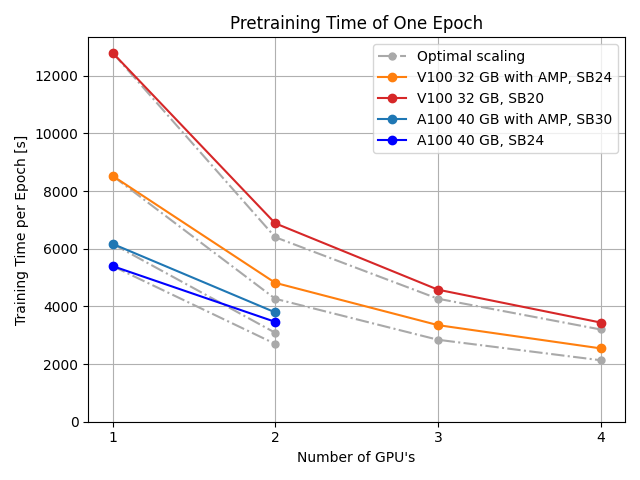
\includegraphics[width=.7\textwidth]{runtime}
    \caption{
        How GPU models, number of GPU's, and AMP influences pretraining runtime.
        Sub-batch size (SB) is included, as it is important for GPU utilization.
        The measurements were taken with da-BERT weights locked.
        The V100's act mostly as expected with close to optimal scaling and AMP decreasing runtime.
        Surprisingly, however, the A100's, while faster, scale poorly and are slower when using AMP.
        The poorly scaling may at least partially be explained by the faster processing time of the A100, causing a relatively larger amount of time to be spent on model synchronization.
        Other differences in hardware and software configurations may also be to blame.
        However, we cannot offer an explanation for AMP being slower on the A100.
        Python 3.8.4 using PyTorch 1.8.1 compiled with CUDA 11.1 was used.
    }
    \label{fig:runtime}
\end{figure}\noindent

\subsubsection{Open Source Software Package}
We publish DaLUKE and all related code under the MIT open source software license \cite{mitlicense}.
All code and documentation is available at \url{https://github.com/peleiden/daluke}.
The pretrained model is available with and without MLM layers at TODO.
The model finetuned on DaNE is available at TODO.
Our software package is \code{pip} installable and runs on Python 3.8 and above.
Simply run `pip install daluke` to install it on your computer.
It allows for using DaLUKE for NER on text files directly from the command line.


\end{document}
